\documentclass{standalone}

\usepackage{tikz}
\usepackage{standalone}
\usetikzlibrary{calc}

\begin{document}

    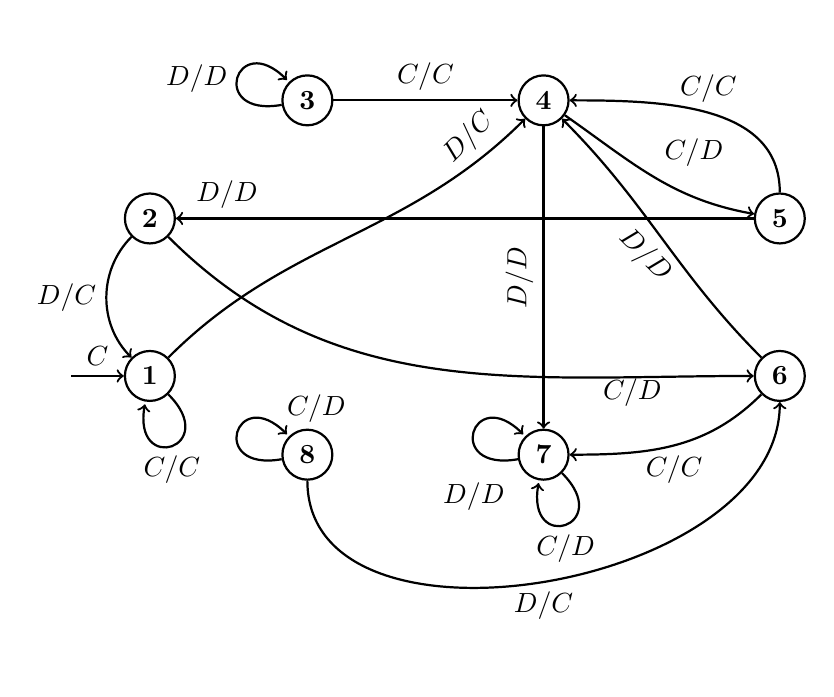
\begin{tikzpicture}

    \tikzstyle{state}=[minimum width=0.5cm, font=\boldmath];

    \node[circle, draw=black, thick]  (0) at (0,0) [state] {$1$};
    \node[circle, draw=black, thick]  (1) at ($(0)+(0,2)$) [state] {$2$};
    \node[circle, draw=black, thick]  (2) at ($(1)+(2,1.5)$) [state] {$3$}; 
    \node[circle, draw=black, thick]  (3) at ($(2)+(3,0)$) [state] {$4$};
    \node[circle, draw=black, thick]  (4) at ($(1)+(8,0)$) [state] {$5$};  
    \node[circle, draw=black, thick]  (5) at ($(0)+(8,0)$) [state] {$6$};
    \node[circle, draw=black, thick]  (6) at ($(3)+(0,-4.5)$) [state] {$7$};
    \node[circle, draw=black, thick]  (7) at ($(2)+(0,-4.5)$) [state] {$8$}; 

    \coordinate[left of=0] (s);

    \draw (s) edge[out=0, in=180, ->, thick] node [above] {$C$} (0);

    \draw (0) edge[out=-45, in=-100, loop, thick] node [below] {$C/C$} (0);
    \draw (6) edge[out=-45, in=-100, loop, thick] node [below] {$C/D$} (6);
    \draw (6) edge[out=190, in=135, loop, thick] node [below, yshift=-0.5cm] {$D/D$} (6);
    \draw (7) edge[out=190, in=135, loop, thick] node [above, xshift=1cm] {$C/D$} (7);
    \draw (2) edge[out=190, in=135, loop, thick] node [left] {$D/D$} (2);

    \draw (2) edge[out=0,in=180,->,thick] node [above] {$C/C$} (3);
    \draw (3) edge[out=-35,in=170,->,thick] node [above right] {$C/D$} (4);
    \draw (5) edge[out=-135,in=0,->,thick] node [below] {$C/C$} (6);

    \draw (0) edge[out=45,in=-135,->,thick] node [above, rotate=45, xshift=2cm, yshift=-0.5cm] {$D/C$} (3);

    \draw (1) edge[out=-45,in=180,->,thick] node [below right, xshift=2cm] {$C/D$} (5);
    \draw (1) edge[out=-135,in=135,->,thick] node [left] {$D/C$} (0);
    \draw (3) edge[out=-90,in=90,->,thick] node [above, rotate=90] {$D/D$} (6);
    \draw (4) edge[out=90,in=0,->,thick] node [above] {$C/C$} (3);
    \draw (4) edge[out=180,in=0,->,thick] node [above left, xshift=-2.5cm] {$D/D$} (1);
    \draw (5) edge[out=135,in=-45,->,thick] node [below, rotate=-45] {$D/D$} (3);
    \draw (7) edge[out=-90,in=-90,->,thick] node [below] {$D/C$} (5);
    \end{tikzpicture}

\end{document}